\documentclass[
BCOR0.7cm,							% Bindekorrektur, bspw. 1 cm
]
{scrbook}

\usepackage{ifpdf} 
\newif\ifpdf
\ifx\pdfoutput\undefined
	\pdffalse              	%normales LaTeX wird ausgef�hrt
\else
	\pdfoutput=1           
	\pdftrue               	%pdfLaTeX wird ausgef�hrt
\fi

\ifpdf %%Einbindung von Grafiken mittels \includegraphics{datei}
	\usepackage[pdftex]{graphicx} %%Grafiken in pdfLaTeX
\else
	\usepackage[dvips]{graphicx} %%Grafiken und normales LaTeX
\fi

\ifpdf
	\pdfinfo
	{
    /Author (Manfred Kindl)                                
    /Title (Abgabetool)     
    /Subject (Benutzerhandbuch Abgabetool)                                    
    /Keywords (Abgabe Abgabetool FH-Complete Technikum-Wien)
	}
\else			
\fi

\usepackage{listings} \lstset{numbers=left, numberstyle=\tiny, numbersep=5pt}
\lstset{language=tex} 

\usepackage[pdftex,colorlinks=true,urlcolor=blue,linkcolor=blue]{hyperref}
\usepackage[ngerman]{babel}		
\usepackage[T1]{fontenc}
\usepackage[latin9]{inputenc}
\usepackage{makeidx}
\usepackage{float}
\usepackage[small,bf]{caption}
\usepackage{fancyhdr}
\usepackage{amssymb,amsmath}
\makeindex

\graphicspath{{../../../../images/}}

\setlength{\tolerance}{2000}
\setlength{\parindent}{0pt}
\setlength{\parskip}{1ex plus 0.5ex minus 0.2ex}
\addtolength{\textheight}{2cm}
\addtolength{\headheight}{2pt}
\setlength{\captionmargin}{20pt}
\floatstyle{plain}
\floatname{example}{Example}

\newfloat{example}{hbtp}{loe}[chapter]
\floatplacement{figure}{hbtp}
\floatplacement{table}{htbp}

\newcommand{\dollar}{\char36}

\newenvironment{info}[1]
{
    \hspace{-10mm}
    \fbox
    {
        \begin{minipage}{1cm}
        
\includegraphics[width=1cm]{icon_info}
        \end{minipage}
        \begin{minipage}{14.5cm}
        #1
        \end{minipage}
    }
}

\newenvironment{achtung}[1]{
    \hspace{-10mm}
    \fbox{
        \begin{minipage}{1cm}
        
\includegraphics[width=1cm]{icon_achtung}
        \end{minipage}
        \begin{minipage}{14.5cm}
        #1
        \end{minipage}
    }
}

\newenvironment{halt}[1]{
    \hspace{-10mm}
    \fbox{
        \begin{minipage}{1cm}
        
\includegraphics[width=1cm]{icon_halt}
        \end{minipage}
        \begin{minipage}{14.5cm}
        #1
        \end{minipage}
    }
}

\newenvironment{idee}[1]{
    \hspace{-10mm}
    \fbox{
        \begin{minipage}{1cm}
        
\includegraphics[width=1cm]{icon_idee}
        \end{minipage}
        \begin{minipage}{14.5cm}
        #1
        \end{minipage}
    }
}


\setlength{\unitlength}{1mm}

\newenvironment{markier}[5]
{    
    \thicklines \put(#2,#3){\vector(#4,#5){5}} \thinlines
    \put(#2,#3){\circle*{5}}
    \put(#2,#3){\textcolor{black}{\circle{5}}\makebox(-10,0){\textcolor{white}{#1}}}
}


\hyphenation{gleich-zeitig para-meter}


\begin{document}

\ifpdf
	\DeclareGraphicsExtensions{.pdf,.jpg,.png}
\else
	\DeclareGraphicsExtensions{.eps}
\fi

\pagestyle{fancyplain}
% Titelseite einbinden

%
% Titelseite, Abstrakt, Danksagung und Inhaltsverzeichnis
%
%% eigene Titelseitengestaltung %%%%%%%%%%%%%%%%%%%%%%%%%%%%%%%%%%%%%%%    

\begin{titlepage}
\begin{center}
\vspace*{30mm} \Huge Abgabetool\\
\vspace*{10mm}
%\large \textsc{Untertitel}

\vfill 
\includegraphics[width=130mm]{cis}\\
\vspace*{20mm}
\textsc{\LARGE{Handbuch f�r Studierende}\\
\vspace*{5mm}
\large{Stand \today}}

	
\vfill \small{FH Technikum Wien}\\

\end{center}
\end{titlepage}



\tableofcontents			% Inhaltsverzeichnis

\frontmatter					% Vorspann (z.B. r�mische Seitenzahlen)

\chapter{Einleitung}
\label{Kapitel Einleitung}

Dieses Handbuch erl�utert die Benutzung und Funktion der Bachelor- und Diplomarbeitsabgabe (kurz Abgabetool) auf der CIS-Seite der FH Technikum Wien.

Das Abgabetool dient zur Interaktion zwischen LektorInnen und Studierenden rund um die Abgabe von Projektarbeiten (Bakk- bzw Diplomarbeiten).
Studierende haben die M�glichkeit, zu definierten Terminen Dokumente hochzuladen.\\
Lektoren k�nnen Abgabetermine (f�r einzelne oder mehrere Studierende) und Abgabefristen definieren und hochgeladene Dokumente betrachten und bewerten.



\mainmatter						% Hauptteil

%% Kapitel Anfang %%%%%%%%%%%%%%%%%%%%%%%%%%%%%%%%%%%%%%%%%%%%%%%%%


\chapter{Abgabetool f�r Studierende}
\label{Kapitel Aufruf}
Der Aufruf der Studierendenoberfl�che erfolgt �ber cis.technikum-wien.at/Mein CIS/Bachelor- und Diplomarbeitsabgabe.

\section{�bersichtsliste der Betreuungen}
In der �bersichtsliste (siehe Abbildung \ref{abgabetool_uebersicht_student}) finden sich alle Betreuungen von Bachelor- und Diplomarbeiten.

\begin {figure}
	\centering
	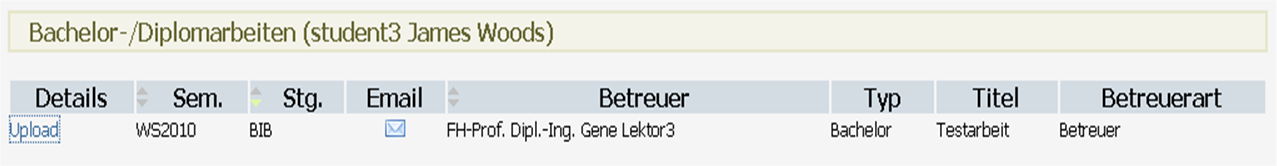
\includegraphics[width=1.0\textwidth]{abgabetool_uebersicht_student}
	\caption{�bersichtsliste der betreuten Arbeiten}
	\label{abgabetool_uebersicht_student}
\end {figure}

\subsection{Aufrufen der Termin�bersicht}
Durch einen Klick auf \textit{Upload} in der ersten Spalte der �bersichtsliste werden die Termindetails im unteren Teil der Seite angezeigt (Siehe Abbildung \ref{abgabetool_termine_student}).

\subsection{E-Mail an den/die Betreuer/Betreuerin}
Durch anklicken des Briefsymbols in der vierten Spalte wird der E-Mailclient ge�ffnet und die Empf�nger- und Absenderadresse sowie \textit{Bachelorarbeitsbetreuung} bzw. \textit{Diplomarbeitsbetreuung} als Betreff werden vorausgef�llt.

\subsection{Aufruf der Anleitung}
Rechts neben der �berschrift \textit{Bachelor- /Diplomarbeitsbetreuungen} befindet sich ein blauer Icon mit einem weissen i. Durch einfaches Klicken darauf kann diese Anleitung als pdf-Datei aufgerufen werden.

\section{Termin�bersicht}

\begin {figure}
	\centering
	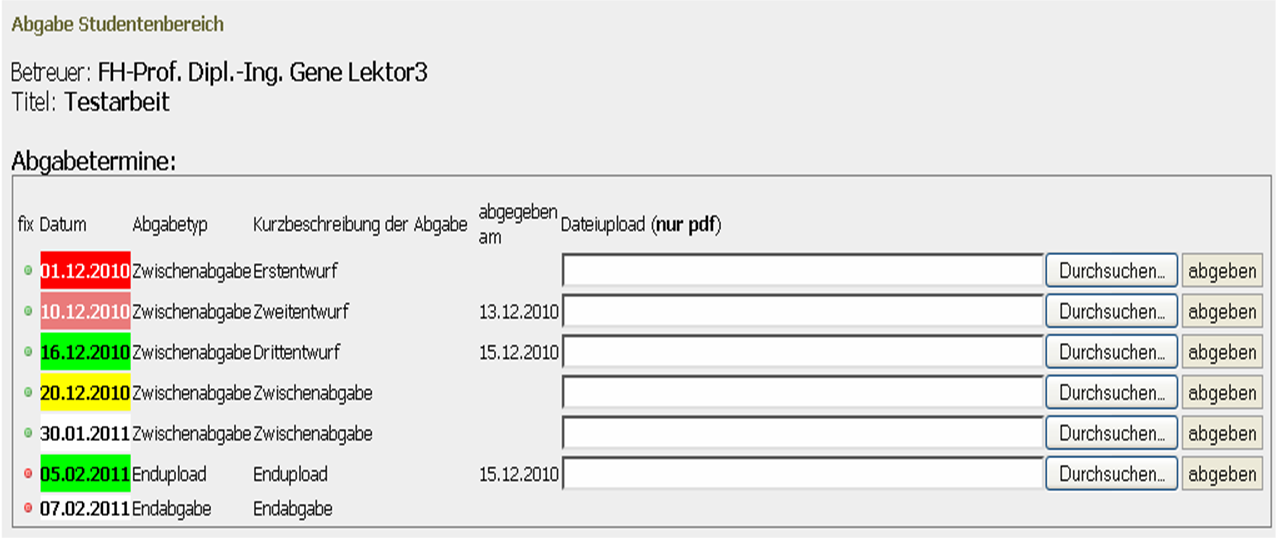
\includegraphics[width=1.0\textwidth]{abgabetool_termine_student}
	\caption{�bersicht der Termine}
	\label{abgabetool_termine_student}
\end {figure}

\subsection{Termine und Dateiupload}

\begin{itemize}
	\item Hier werden Zeilenweise die verschiedenen Termine (Erstentwurf, Zwischenabgabe, Endupload,...) mit einer kurzen Beschreibung angezeigt. 
	\item Die Farbcodierung weist auf den Terminstatus hin (siehe Abschnitt \ref{farbcode})
	\item Klicken Sie beim jeweiligen Termin auf \textit{Durchsuchen} um Ihre Festplatte nach der gew�nschten Datei zu durchsuchen. Klicken Sie danach auf \textit{abgeben} um die Datei wegzuschicken. Ihr/e Betreuer/in wird automatisch per E-Mail �ber die erfolgte Abgabe informiert. Wenn Sie erneut eine Datei hochladen, wird die bestehende Datei �berschrieben.	
	\item Die Studiengangsassistenz kann fixe Termine vergeben, erkennbar an dem roten Bullet in der Spalte \textit{fix}. Liegt ein fixer Termin in der Vergangenheit, k�nnen Sie zu diesem nichts mehr hochladen. Soll dennoch etwas hochgeladen werden, m�ssen Sie bei der Studiengangsassistenz um eine Korrektur des Termins ansuchen.
	
	\info{Es k�nnen derzeit nur Dateien im Format PDF hochgeladen werden}
\end{itemize}

\subsection{Farbcode}
\label{farbcode}

\begin{itemize}
	\item wei�:	"normaler" Termin
	\item gelb:	Termin innerhalb der n�chsten 12 Tage
	\item rot:	Termin �berschritten
	\item gr�n:	Abgabe erfolgt
	\item hellrot: Abgabe nach Termin 
\end{itemize}

\subsection{Zusatzdaten beim Endupload}
Am Termin vom Typ \textit{Endupload} erscheint nach dem Upload ein Formular (siehe Abbildung \ref{abgabetool_zusatzdaten_student}), in dem Sie dazu aufgefordert werden, zus�tzliche Daten f�r die Publikationsdatenbank einzugeben. Diese werden ebenfalls vom Betreuer/der Betreuerin auf Vollst�ndigkeit kontrolliert.
\begin{itemize}
	\item Sprache der Arbeit: Sprache in der die Arbeit verfasst wurde
	\item Kontrollierte Schlagw�rter: Hier k�nnen mit Hilfe eines Schlagwortdienstes, kontrollierte Schlagw�rter hinzugef�gt werden. Siehe Schlagwortdienst
	\item Dt. Schlagw�rter: Schlagw�rter zur Kategorisierung der Arbeit
	\item Engl. Schlagw�rter: Englische Schlagw�rter zur Kategorisierung der Arbeit 
	\item Abstract: Abstract der Arbeit
	\item Abstract engl.: Englischer Abstract der Arbeit
	\item Seitenanzahl: Anzahl der Seiten der Arbeit
	\item Eidesstattliche Erkl�rung: Akzeptieren der Erkl�rung
\end{itemize}
\begin {figure}
	\centering
	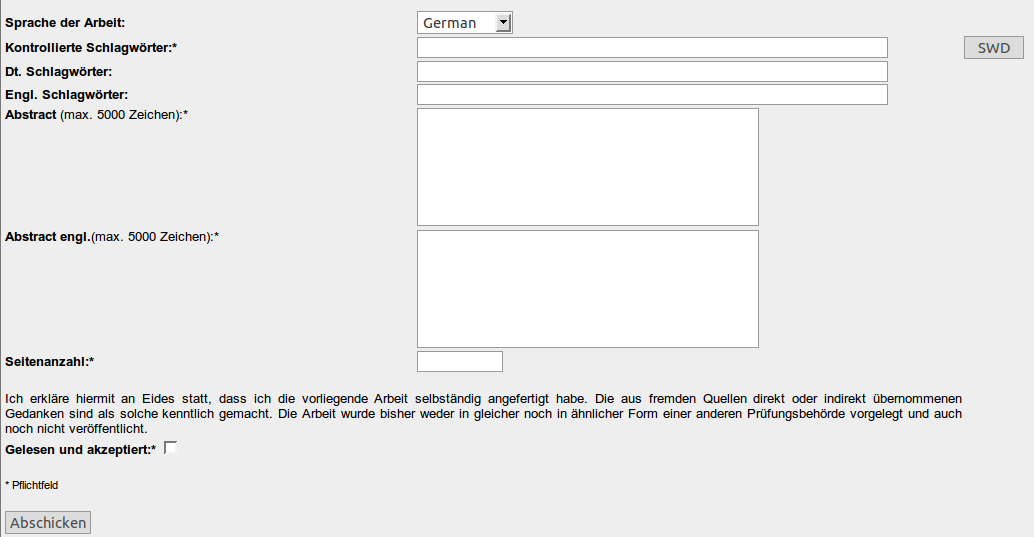
\includegraphics[width=1.0\textwidth]{abgabetool_zusatzdaten_student}
	\caption{Zusatzdaten nach dem Endupload}
	\label{abgabetool_zusatzdaten_student}
\end {figure}

\subsection{Schlagwortdienst}
Kontrollierte Schlagw�rter k�nnen mit Hilfe eines Schlagwortdienstes eingetragen werden.\\
Durch einen klick auf den Button SWD wird der Schlagwortdienst ge�ffnet. 
Sie werden auf eine externe Seite weitergeleitet.
\begin {figure}
	\centering
	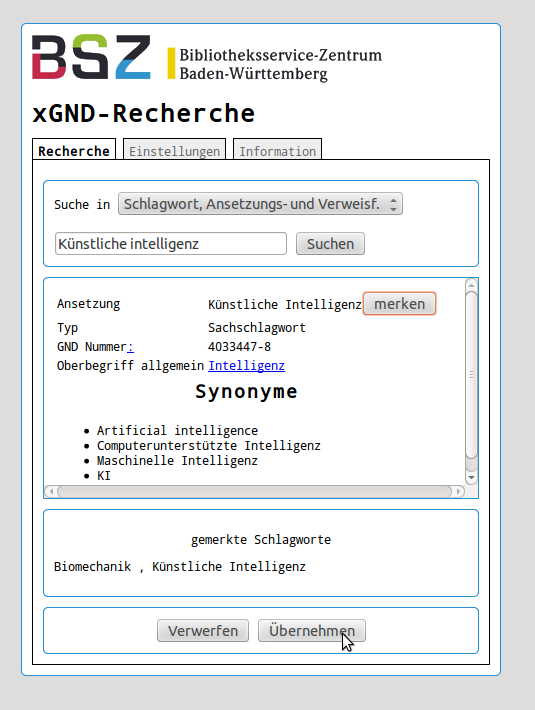
\includegraphics[width=0.5\textwidth]{abgabetool_swd}
	\caption{SWD}
	\label{SWD}
\end {figure}
\\
�ber die Suchfunktion kann nach Schlagw�rtern gesucht werden.
\\Klicken Sie auf den Button ''merken'' um Schlagw�rter auszuw�hlen.
\\Wenn Sie alle Schlagw�rter hinzugef�gt haben k�nnen Sie diese �ber den Button ''�bernehmen'' in das Abgabe-Formular �bertragen.
siehe Abbildung \ref{SWD}

\subsection{Probleme beim Upload}
Falls beim Upload der Datei Probleme auftreten kann dies folgende Gr�nde haben:

\begin{itemize}
	\item Die Dateigr��e darf maximal 15 MB betragen.
	\item Die hochzuladende Datei muss im PDF Format vorliegen. Der Upload von anderen Dateitypen ist nicht m�glich
	\item Deaktivieren Sie eventuell installierte Addons Ihres Browsers (Adblocker, NoScript, etc)
	\item Stellen Sie sicher, dass Javascript aktiviert ist
	\item Versuchen Sie die Arbeit mit einem anderen Browser hochzuladen (zB Firefox)
\end{itemize}


%% Kapitel Ende   %%%%%%%%%%%%%%%%%%%%%%%%%%%%%%%%%%%%%%%%%%%%%%%%%
\appendix							% Beginn des Anhangs
%\chapter{Schluss}
%\listoftables				% Tabellenverzeichnis
%\listoffigures				% Abbildungsverzeichnis

\end{document}
